\documentclass[xcolor=dvipsnames,10pt]{beamer}
\usepackage[utf8]{inputenc}
\usepackage[T1]{fontenc}
\usepackage[brazilian]{babel}
\usepackage{etoolbox}
\usepackage{graphicx}
\usepackage{ragged2e}
\usepackage{tikz}

\makeatletter
\patchcmd{\beamer@sectionintoc}{\vskip1.5em}{\vskip0.5em}{}{}
\makeatother

\usefonttheme[professional]{serif}

\justifying

%----------------------------------------------------------------------------------------------------------------------------------

% JUSTIFICAR TEXTO DAS LISTAS DE ITENS

\makeatletter
\renewcommand{\itemize}[1][]{%
  \beamer@ifempty{#1}{}{\def\beamer@defaultospec{#1}}%
  \ifnum \@itemdepth >2\relax\@toodeep\else
    \advance\@itemdepth\@ne
    \beamer@computepref\@itemdepth% sets \beameritemnestingprefix
    \usebeamerfont{itemize/enumerate \beameritemnestingprefix body}%
    \usebeamercolor[fg]{itemize/enumerate \beameritemnestingprefix body}%
    \usebeamertemplate{itemize/enumerate \beameritemnestingprefix body begin}%
    \list
      {\usebeamertemplate{itemize \beameritemnestingprefix item}}
      {\def\makelabel##1{%
          {%
            \hss\llap{{%
                \usebeamerfont*{itemize \beameritemnestingprefix item}%
                \usebeamercolor[fg]{itemize \beameritemnestingprefix item}##1}}%
          }%
        }%
      }
  \fi%
  \beamer@cramped%
  \justifying% NEW
  %\raggedright% ORIGINAL
  \beamer@firstlineitemizeunskip%
}
\makeatother

%%%%%%%%%%%%%%%%%%%%%%%%%%%%

%%%%%%%%%%%%%%%%%%%%%%%%%%%%%%%%%%%%%%%%%%%%%%%%%%%%%%%%%%%%%%%%%%%%%%%%%%%%%%%%
%COR DO TEMPLATE SEMELHANTE AO LOGO
%%%%%%%%%%%%%%%%%%%%%%%%%%%%%%%%%%%%%%%%%%%%%%%%%%%%%%%%%%%%%%%%%%%%%%%%%%%%%%%%
\definecolor{laranja}{rgb}{0.95703125,0.5859375,0.30859375}

%%%%%%%%%%%%%%%%%%%%%%%%%%%%%%%%%%%%%%%%%%%%%%%%%%%%%%%%%%%%%%%%%%%%%%%%%%%%%%%%
%CORES E ESTRUTURAS DE ELEMENTOS DIVERSOS
%%%%%%%%%%%%%%%%%%%%%%%%%%%%%%%%%%%%%%%%%%%%%%%%%%%%%%%%%%%%%%%%%%%%%%%%%%%%%%%%
\setbeamercolor{frametitle}{fg=black}
\setbeamercolor{headline}{fg=black}
\setbeamercolor{footline}{fg=black}
\setbeamercolor{block body}{use=structure,bg=white}
\setbeamercolor{block title}{use=structure,bg=laranja,fg=black}
\setbeamercolor{item}{fg=laranja}
\setbeamercolor{alerted text}{fg=laranja}
\setbeamercolor{section in toc}{fg=black}
\setbeamercolor{title}{fg=black}
\setbeamercolor{subtitle}{fg=black}
\setbeamertemplate{blocks}[rounded][shadow=true]

%%%%%%%%%%%%%%%%%%%%%%%%%%%%%%%%%%%%%%%%%%%%%%%%%%%%%%%%%%%%%%%%%%%%%%%%%%%%%%%%
%PROPRIEDADES VISUAIS DE ELEMENTOS DIVERSOS
%%%%%%%%%%%%%%%%%%%%%%%%%%%%%%%%%%%%%%%%%%%%%%%%%%%%%%%%%%%%%%%%%%%%%%%%%%%%%%%%
\useoutertheme[]{default}
\addtobeamertemplate{block begin}{}{\justifying} % Justify all blocks

\setbeamertemplate{section in toc}[circle]
\setbeamertemplate{subsection in toc}[square]
\setbeamertemplate{itemize item}{$\bullet$}
\setbeamertemplate{navigation symbols}{}
\setbeamercovered{invisible}
\setbeamertemplate{sections in toc}[ball]

%%%%%%%%%%%%%%%%%%%%%%%%%%%%%%%%%%%%%%%%%%%%%%%%%%%%%%%%%%%%%%%%%%%%%%%%%%%%%%%%
%LOGOS POSICIONADOS NO RODAPÉ
%%%%%%%%%%%%%%%%%%%%%%%%%%%%%%%%%%%%%%%%%%%%%%%%%%%%%%%%%%%%%%%%%%%%%%%%%%%%%%%%
\setbeamertemplate{footline}{
  \vspace{0.5em}
  \tikz \fill [laranja] (0,0) rectangle (15, 2pt);

\vspace{-1.3em}
\begin{center}

\includegraphics[height=0.50cm]{logo-iff.png}\hspace{0.4em}

\includegraphics[height=0.50cm]{logo-iprj.png}\hspace{0.4em}

\includegraphics[height=0.50cm]{logo-uerj.png}\hspace{0.4em}

\includegraphics[height=0.50cm]{logo-uesc.png}\hspace{0.4em}

\includegraphics[height=0.50cm]{logo-capes.png}\hspace{0.4em}

\includegraphics[height=0.50cm]{logo-cnpq.png}\hspace{0.4em}

\includegraphics[height=0.50cm]{logo-faperj.png}\hspace{0.4em}

\includegraphics[height=0.50cm]{logo-buzios.png}\vspace{-0.5em}
\end{center}
}

%%%%%%%%%%%%%%%%%%%%%%%%%%%%%%%%%%%%%%%%%%%%%%%%%%%%%%%%%%%%%%%%%%%%%%%%%%%%%%%%
%LOGO DO EVENTO COMO TÍTULO DE TODOS OS SLIDES
%%%%%%%%%%%%%%%%%%%%%%%%%%%%%%%%%%%%%%%%%%%%%%%%%%%%%%%%%%%%%%%%%%%%%%%%%%%%%%%%
\setbeamertemplate{headline}{

\vspace{-1em}
\begin{center}

\includegraphics[width=0.5	\textwidth]{logo-evento.png}
\end{center}
}
%%%%%%%%%%%%%%%%%%%%%%%%%%%%%%%%%%%%%%%%%%%%%%%%%%%%%%%%%%%%%%%%%%%%%%%%%%%%%%%%
% INICIO DOS SLIDES
%%%%%%%%%%%%%%%%%%%%%%%%%%%%%%%%%%%%%%%%%%%%%%%%%%%%%%%%%%%%%%%%%%%%%%%%%%%%%%%%
\title{\textbf{\small COMPARISON BETWEEN DIFFERENCIAL EVOLUTION AND SIMULATED ANNEALING ALGORITHMS APPLIED TO THE CONSTRUCTAL DESIGN OF THE DOUBLE-T SHAPED CAVITIES
}}

\author{\small G. V. Gonzales,  L. A. Isoldi, L. A. O. Rocha, E. D. dos Santos e \\
A. J. Silva Neto}
\institute{\vspace{-0.3cm}\scriptsize Programa de Pós-Graduação em Modelagem Computacional - FURG}
%%\subtitle{\vspace{0.3cm}\small Métodos Computacionais\vspace{-0.3cm}}
\date{\vspace{-0.8cm}\scriptsize Outubro de 2018}
\begin{document}

\frame{\titlepage}
\frame{\tableofcontents}

\section{Introdução}
\subsection{Motivação e Objetivos}
\begin{frame}{}
	\begin{block}{\textbf{\textsc{INTRODUÇÃO: Motivação}}}s
	Com a miniaturização dos circuitos eletrônicos e desenvolvimento de dispositivos cada vez mais compactos, técnicas tradicionais de troca térmica por convecção forçada não são mais suportadas. Alternativas apontam para cavidades ou caminhos com material de alta condutibilidade.
	\end{block}
\end{frame}
\begin{frame}{}
	\begin{block}{\textbf{\textsc{INTRODUÇÃO: Objetivos}}}
		\begin{itemize}
		\item Otimizar parcialmente uma cavidade em forma de Duplo-T;
		\item Comparar os resultados de duas meta-heurísticas aplicadas ao problema
		\item Analisar diferentes parâmetros de cada algoritmo;
		\item Avaliar estatisticamente as diferenças entre os resultados da reprodução dos efeitos dos graus de liberdade sobre a geometria ótima e a temperatura máxima minimizada;
		\item Recomendar não só o algoritmo mas também a configuração de parâmetros mais adequada ao problema de otimização;
	\end{itemize}
	\end{block}
\end{frame}

\subsection{Breve Estado da Arte}
	\begin{frame}{}
	\begin{block}{\textbf{\textsc{INTRODUÇÃO: Breve Estado da Arte}}}
		\begin{itemize}
		\item Cavidade em formato de "C" e "T"  em Biserni et. al. (2004). 
		\item Cavidade em forma de "H"  em Biserni et. al.(2007).
		\item Cavidade em forma de "Y"  em (Lorenzini et. al.(2011).
		\item Cavidade em forma de "Y" aplicação do Algoritmo Genético  em Lorenzini et. al.(2014).
		\item Comparação entre aplicação do SA com GA na otimização da cavidade em forma de Y  em Gonzales et. al.(2015a).
		\item Otimização parcial até 3 graus de liberdade da cavidade em duplo-T  em Gonzales et. al. (2015b).
	\end{itemize}
	\end{block}
\end{frame}

\section{Modelagem Matemática e Numérica}
\begin{frame}{}
\begin{block}{\textbf{\textsc{Modelagem Matemática e Numérica}}}
		\textbf{Hipóteses Simplificativas:}
		\begin{enumerate}
			\item Regime Permanente
			\item Geração uniforme de calor
			\item Condutividade térmica constante
			\item Domínio bidimensional
		\end{enumerate}
	
		\begin{equation}
		\frac{\partial}{\partial x}\left( k\frac{\partial \theta}{\partial x}\right)+
		\frac{\partial}{\partial y}\left(k\frac{\partial \theta}{\partial y}\right)+
		\frac{\partial}{\partial z}\left(k\frac{\partial \theta}{\partial z}\right)+ 
		q^{'''}=\rho C_p\frac{\partial \theta}{\partial t}\label{calor}
		\end{equation}
		\begin{equation}
		\frac{\partial ^{2} \theta}{\partial x^{2}}+\frac{\partial ^{2} \theta}{\partial y^{2}}+\frac{q^{'''}}{k}=0\label{calor}
		\end{equation}
	\end{block} 
\end{frame}
\begin{frame}
%%\begin{block}{\textbf{MODELAGEM MATEMÁTICA}}
\begin{figure}[h!]
			\centering
			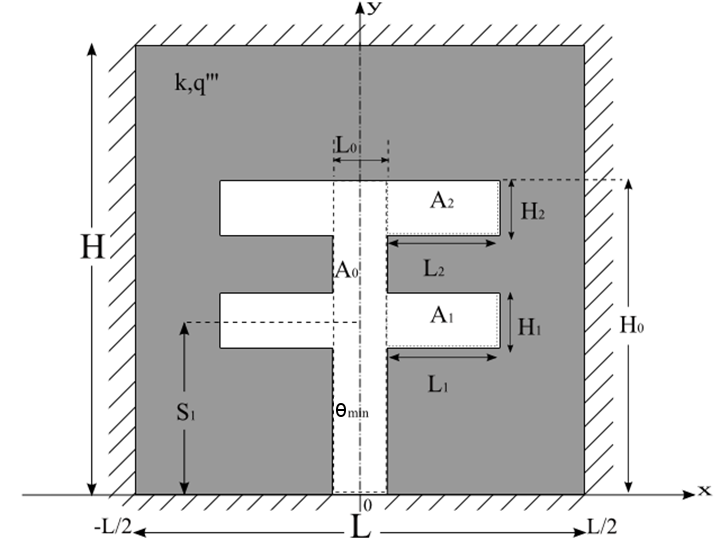
\includegraphics[width=0.66\linewidth]{../../imgs/duplo_t.png}
			\caption{ {\small Domínio Computacional da Cavidade em Forma de Duplo-T.}}
			\label{figure01}
		\end{figure}
%%\end{block}
\end{frame}
\begin{frame}{}
	\begin{block}{\textbf{\textsc{Modelagem Matemática e Numérica}}}
	\textbf{Restrições: }
		\begin{equation}
			A = HL \label{area_total}
		\end{equation}
		\begin{equation}
			A_{c} = A_{0} + 2A_{1} + 2A_{2} \label{area_cavidade}
		\end{equation}\begin{equation}
			\phi_{c} = A_{c}/A \label{fi}
		\end{equation}
		
	\end{block} 
\end{frame}
\begin{frame}
\begin{block}{\textbf{\textsc{Modelagem Matemática e Numérica}}}
\textbf{Adimensionalização do Problema:}
\begin{equation}
			\tilde{\theta} = \frac{\theta - \theta_{min}}{q^{'''}\cdot\frac{A}{k}}\label{tadim}
		\end{equation}
		\begin{equation}
				\tilde{x},\tilde{y},\tilde{H}_{0},\tilde{H}_{1},\tilde{H}_{2},\tilde{L}_{0},\tilde{L}_{1},\tilde{L}_{2},\tilde{H},\tilde{L},\tilde{S}_{1} = \frac{x,y,H_{0},H_{1},H_{2},L_{0},L_{1},L_{2},H,L,S_{1}}{A^{1/2}}\label{vadim}
		\end{equation}
		\begin{equation}
				\frac{\partial ^{2}\tilde{\theta}}{\partial \tilde{x}^{2}}+\frac{\partial ^{2} \tilde{\theta}}{\partial \tilde{y}^{2}}+1=0\label{calor}
		\end{equation}
		\begin{equation}
			\tilde{\theta}_{max}=\frac{\theta_{max}-\theta_{min}}{q^{'''}\cdot\frac{A}{k}}\label{fo}
		\end{equation}
		\end{block}
\end{frame}
\begin{frame}
\begin{block}{\textbf{\textsc{Modelagem Matemática e Numérica}}}
\justifying
	\setlength{\parindent}{1cm}
		A função representada pela Eq. \ref{fo} é resolvida numericamente através da resolução da Eq. \ref{calor} para a determinação dos os campos de temperatura em todo o domínio computacional para diferentes configurações de ($H$, $L$, $H_{0}$, $L_{0}$, $H_{1}$, $L_{1}$, $H_{2}$, $L_{2}$ e $S_{1}$) e calculando o $\tilde{\theta}_{max}$ para minimizar o seu valor através da variação da configuração geométrica.\\ A solução numérica é dada pela aplicação do método de Elementos Finitos (FEM), baseado em elementos triangulares, desenvolvido no ambiente MATLAB$^{\tiny ®}$, com o pacote PDE (partial-differential-equations) toolbox.\\ A malha utilizada é não-uniforme em ambos eixos $x$ e $y$, e varia de uma geometria para outra. O tamanho é de  80649 mil elementos.
	\end{block}
\end{frame}
\section{Otimização}
\begin{frame}
	\begin{block}{\textbf{\textsc{Otimização}}}
	\justifying
	\setlength{\parindent}{1cm}
	A metodologia de otimização aplicada neste trabalho utiliza-se do método Constructal Design associado as meta-heurísticas de Evolução Diferencial e Recozimento Simulado. 
	\begin{itemize}
		\item \textbf{Constructal Desing}: para definição dos objetivos, restrições, graus de liberdade e espaço de busca.
		\item \textbf{Algoritmos de Otimização}: neste trabalho aplicamos os algoritmos de Evolução Diferencial e Recozimento Simulado  para a obtenção das geometrias ótimas.
		\item \textbf{Comparação dos Resultados}: São utilzidos os valores de média entre 30 execuções de cada algoritmo e comparados com os melhores resultados encontrados entre todas as rodadas.
	\end{itemize}
	\end{block}
\end{frame}
\subsection{Design Construtal}
\begin{frame}{}
	\begin{block}{\textbf{Constructal Design}}
		\justifying
		\setlength{\parindent}{1cm}
		\textbf{Definição dos Graus de Liberdade e Restrições:}
		\begin{itemize}
			\item Nove variáveis ($H$, $L$, $H_{0}$, $L_{0}$, $H_{1}$, $L_{1}$, $H_{2}$, $L_{2}$ e $S_{1}$);
			\item Quatro restrições ($A$,$A_c$,$A_1$ e $A_2$);
			\begin{equation}
				\phi_c = A_c/A= \tilde{H_{0}}\tilde{L_{0}}+2\phi_1+2\phi_2
			\end{equation}
			\begin{equation}
				\phi_1 = \tilde{H_{1}}\tilde{L_{1}} 
			\end{equation}
			\begin{equation}
				\phi_2 = \tilde{H_{2}}\tilde{L_{2}}
			\end{equation}
			\item Temos cinco graus de liberdade ($H/L$, $H_{0}/L_{0}$, $H_{1}/L_{1}$, $H_{2}/L_{2}$ e $S_{1}/H_{0}$) para o fechamento das equações;
			
		\end{itemize}
	\end{block}
\end{frame}
\begin{frame}{}
	\begin{block}{\textbf{Constructal Design}}
		\justifying
		\setlength{\parindent}{1cm}
		\begin{itemize}
\item Durante o processo de otimização, foram mantidos constantes os valores das restrições ($\phi_c = 0.1,  \phi_1 = \phi_2 = 0.015$) 
\item O grau de liberdade $H/L$ foi variado entre $0.3 =< H/L<= 30$
			\item Foram variados os graus de liberdade: $H_{0}/L_{0}$, $H_{1}/L_{1}$, $H_{2}/L_{2}$ e $S_{1}/H_{0}$.

		\end{itemize}
	\end{block}
\end{frame}

\subsection{Configuração dos Algoritmos}
\begin{frame}{}
\textbf{Configurações dos Algoritmos}
			\begin{table}[H] % !htbp
			\caption{Versões do Algoritmo Differential Evolution. }
			\label{table1}
			\vspace{5pt}
			\centering{}
			\begin{tabular*}{\textwidth}{@{\extracolsep{\fill}}c|c|c|c|c|c|c|c|c|c}        % {0.8\textwidth}
			\hline
				& DE1 & DE2 & DE3 & DE4 \tabularnewline
			\hline
				$F$ & 1,5 & 2,0 & 1,5 & 2,0\tabularnewline
			\hline 
				Taxa Cruz. & 0,7 & 0,9 & 0,7 & 0,9\tabularnewline
			\hline
				Tipo & rand/1/bin & rand/1/bin & best/2/bin & best/2/bin \tabularnewline
			\hline
				Iter & 25 G x 20 I = 500 & - & - & - \tabularnewline
				\hline
			\end{tabular*}
			\end{table}
\end{frame}	
\begin{frame}
\textbf{Configurações dos Algoritmos}
			\begin{table}[H] % !htbp
			\caption{Versões do Algoritmo Simulated Annealing. }
			\label{table1}
			\vspace{5pt}
			\centering{}
			\begin{tabular*}{\textwidth}{@{\extracolsep{\fill}}c|c|c|c|c|c|c|c|c|c}        % {0.8\textwidth}	
			\hline
				& SA{\_}E & SA{\_}B & SA{\_}BE & SA{\_}C1 & SA{\_}C2\tabularnewline
			\hline
				C. Schedule & Exponencial & Boltz & BoltzExp & ConstExp1 &  
ConstExp2\tabularnewline
			\hline 
				StallIterLimit. & 250 & - & - & -&-\tabularnewline
			\hline
				Reannealing & 150 & - & - & - & -\tabularnewline
			\hline
				Iter & 500 & - & - & - & -\tabularnewline
			\hline
			\end{tabular*}
			\end{table}	
	\end{frame}


\section{Resultados}

\begin{frame}

\begin{block}{Resultados}
Resultado...
\end{block}

\end{frame}

\section{Conclusão}

\begin{frame}

\begin{block}{Conclusão}
Conclusão...
\end{block}

\end{frame}

\section{Referências}

\begin{frame}

\begin{block}{Referências}
Referências...
\end{block}

\end{frame}

\section{Agradecimentos}

\begin{frame}

\begin{block}{Agradecimentos}
Agradecimentos...
\end{block}

\end{frame}

\end{document}